% ============================================================
% LLM-BLM 実験結果レポート
% コンパイル：tectonic -X compile LLM-BLM_実験結果レポート.tex   （XeTeX 系。資料集/ の直下で実行する）
% 図は LLM-BLM_実験結果レポート_図/（作成スクリプト/figs.py が experiments/H0x/results から作る）
% 設計は『LLM-BLM_実験仮説』、数値の出どころは experiments/H0x/results/summary.json と findings.md
% ============================================================
\documentclass[xelatex,ja=standard,jafont=haranoaji,a4paper,10pt,openany]{bxjsreport}
\setpagelayout*{left=24mm,right=24mm,top=24mm,bottom=26mm,footskip=11mm}

\usepackage{amsmath,amssymb,mathtools,bm}
\usepackage{booktabs,array,multirow,longtable}
\usepackage{graphicx}
\usepackage{adjustbox}
\usepackage{xcolor}
\usepackage{tikz}
\usetikzlibrary{arrows.meta,positioning,calc,fit}
\usepackage{listings}
\usepackage{enumitem}
\usepackage{caption}
\usepackage[most]{tcolorbox}
\usepackage[hidelinks,bookmarksnumbered]{hyperref}
\pdfstringdefDisableCommands{\def\Omega{Ω}\def\tau{τ}\def\Sigma{Σ}\def\Pi{Π}\def\mu{μ}\def\delta{δ}\def\T{ᵀ}}

\graphicspath{{LLM-BLM_実験結果レポート_図/}}

\definecolor{c1}{HTML}{2A78D6}
\definecolor{c2}{HTML}{EB6834}
\definecolor{c3}{HTML}{1BAF7A}
\definecolor{c4}{HTML}{EDA100}
\definecolor{c7}{HTML}{6250D6}
\definecolor{ink2}{HTML}{52514E}
\definecolor{soft1}{HTML}{E4EEF9}
\definecolor{soft2}{HTML}{FBEEDF}
\definecolor{soft3}{HTML}{E3F3E9}
\definecolor{soft4}{HTML}{EEE8FA}
\definecolor{soft5}{HTML}{FDF3DA}

\newcommand{\code}[1]{\texttt{#1}}
\newcommand{\SP}{S\&P500}
\newcommand{\T}{^{\top}}
\newcommand{\muBL}{\mu_{\mathrm{BL}}}
\newcommand{\wmkt}{w_{\mathrm{mkt}}}
\newcommand{\IC}{\mathrm{IC}}
\newcommand{\TE}{\mathrm{TE}}
\newcommand{\figref}[1]{図~\ref{#1}}
\newcommand{\tabref}[1]{表~\ref{#1}}
\newcommand{\chapref}[1]{第~\ref{#1}~章}
\newcommand{\secref}[1]{\ref{#1}~節}

\setlist[itemize]{leftmargin=1.6em,itemsep=0.2em,topsep=0.4em}
\setlist[enumerate]{leftmargin=1.8em,itemsep=0.2em,topsep=0.4em}
\captionsetup{font=small,labelfont=bf,skip=6pt}
\renewcommand{\arraystretch}{1.2}
\setlength{\LTpre}{6pt}
\setlength{\LTpost}{6pt}

\makeatletter
\def\@makechapterhead#1{\vspace*{0.3\Cvs}{\parindent\z@\raggedright\normalfont
  \ifnum\c@secnumdepth>\m@ne\if@mainmatter{\Large\headfont\@chapapp\thechapter\@chappos}\par\nobreak\vskip0.4\Cvs\fi\fi
  \interlinepenalty\@M\LARGE\headfont #1\par\nobreak\vskip 1.5\Cvs}}
\def\@makeschapterhead#1{\vspace*{0.3\Cvs}{\parindent\z@\raggedright\normalfont
  \interlinepenalty\@M\LARGE\headfont #1\par\nobreak\vskip 1.5\Cvs}}
\makeatother

\newtcolorbox{keybox}[1][要点]{enhanced,breakable,colback=soft1,colframe=c1,boxrule=0.5pt,arc=2pt,
  left=8pt,right=8pt,top=6pt,bottom=6pt,title={#1},fonttitle=\sffamily\bfseries\small,coltitle=white}
\newtcolorbox{notebox}[1][注意]{enhanced,breakable,colback=soft2,colframe=c2,boxrule=0.5pt,arc=2pt,
  left=8pt,right=8pt,top=6pt,bottom=6pt,title={#1},fonttitle=\sffamily\bfseries\small,coltitle=white}
\newtcolorbox{verdict}[1][判定]{enhanced,breakable,colback=soft4,colframe=c7,boxrule=0.5pt,arc=2pt,
  left=8pt,right=8pt,top=6pt,bottom=6pt,title={#1},fonttitle=\sffamily\bfseries\small,coltitle=white}

\tikzset{
  box/.style={draw=#1,fill=#1!8,rounded corners=2pt,align=center,font=\footnotesize,inner sep=4pt,
              minimum height=10mm,text width=23mm},
  arr/.style={-{Stealth[length=2mm]},color=ink2,line width=0.6pt},
}

\title{LLM-BLM 実験結果レポート\\[6pt]
  \large LLM のビューは Black-Litterman モデルと単純な統計に\\追加の価値を生むか：7 つの仮説の検証}
\author{実験の結果の報告書}
\date{2026 年 10 月 17 日}

\begin{document}
\maketitle

% ============================================================
\chapter*{概要}
\addcontentsline{toc}{chapter}{概要}

『LLM-BLM 実験仮説』（以下、設計書）で立てた 7 つの仮説を、設計書で決めた指標と判定の基準のとおりに検証した。評価の期間は 2024 年 3 月末から 2026 年 8 月末の判断日 30 か月、対象は各時点の \SP{} の構成銘柄（月平均 489 銘柄）、予想に使った LLM は gpt-4o-mini（知識の期限が評価期間より前）だけである。API の費用は合計 6.72 ドル（18,237 リクエスト）だった。結果は、別の 2 つのモデル（gpt-5.3-codex と gemini-3.1-pro）にも読ませて考察を深め、指摘のうち確かめられるものは追加の計算で確かめた（\chapref{ch:review}）。

\begin{keybox}[主な結論]
\begin{itemize}
\item \textbf{LLM の数値予想（既存の実行 1）は、入力の写しである。}予想の 81\% は、渡した月の平均と散らばりの直線の関数で説明でき、その写しを除いた LLM に固有の部分の IC は $-0.004$（95\% 区間 $-0.036$〜$+0.027$）だった。LLM の予想と同じ当たり具合（IC $+0.05$）は、「先月の平均リターン」をそのまま使っても得られる（H02、支持）。
\item \textbf{BLM の計算は、$\Omega$ を当たり具合で較正し $\Sigma$ に比例させれば、設計どおりに働く。}採用率は設定どおり、比率は時価総額加重を少し動かす形（実質 47 銘柄、実績の TE 4.2\%）になった。しかし、その成績（コスト控除後 年率 $+0.5\%$）は、予想を銘柄の間でランダムに並べ替えたビュー 200 回と区別できない（片側 $p=0.10$）（H04、支持）。
\item \textbf{LLM のビューの「ベータの傾き」は、相対ビューにしても消えない。}市場が上がった月に高ベータの銘柄が上がり、LLM がそれをなぞるため、銘柄の間の予想の差そのものがベータに傾く（H03、支持されなかった）。
\item \textbf{文章だけを渡すと、LLM は数字のなぞりから離れる。}月次レポートの文章だけでは、市場の点数と直近 1 か月のリターンの順位相関が $+0.77$ から $+0.05$ に下がった（H05）。決算発表文 5,429 本の点数も、直近のリターンとはほぼ無相関（$+0.08$）で、業績の伸び（$+0.41$）に沿った。ただし、事前に決めた検定では、どちらも 30 か月で当たることを確かめられなかった（決算発表文の IC $+0.033$、$t$ 1.57。数値を統制した係数の $t$ 0.97）（H06、支持されなかった）。月ごとの IC の自己相関を考慮した Newey--West の $t$ 値では、決算発表文の IC は $t$ 2.32（$p=0.028$）になり、探索的には有意だった。LLM を使う意味が残っているのは、この「文章からの点数」だけである。
\item \textbf{フィードバックの LLM は、予想を良くしなかった。}自分の過去の成績の要約を渡しても IC は上がらず（差 $+0.011$、$t$ 0.76）、楽観の偏りはかえって 2.4 倍になった。前月の外れを渡すと、予想を雑音の 2 倍以上動かした（H07、証拠不足）。
\item 計算上の問題として、元論文の最適化（SciPy の SLSQP）は、入力のごく小さな違いで止まる位置が変わり、結果を再現できないことを確かめた（H01）。
\end{itemize}
\end{keybox}

\textbf{推奨}：LLM に数値のリターンを予想させる構成はやめ、(1) BLM は当たり具合で較正した $\Omega\propto\Sigma$ と TE の上限で「安全に何もしない」形を土台にし、(2) LLM の役割を文章からの情報の抽出に絞り、その点数の価値は較正の傾きが正で安定するまでビューに入れない（入れても採用率は自動で 0 に近くなる）。30 か月の評価期間では、LLM にも統計モデルにも、ビューとしての価値は確かめられなかった。詳しくは\chapref{ch:recommend}。

\setcounter{tocdepth}{1}
{\small\tableofcontents}

% ============================================================
\chapter{研究の目的と背景}\label{ch:intro}

本研究の目的は、LLM を使うこと自体を正当化することではない。LLM が、既存の Black-Litterman モデル（BLM）や単純な統計の方法に対して、本当に追加の価値を生むかを確かめることである。

既存の資料（『総合報告書』と『BLM ビューとリスクのコツ』）は、次のことを報告していた。

\begin{itemize}
\item 元論文の計算では、BLM が LLM の予想を中央値で 99.9\% 採用し、市場の均衡がほとんど使われていない。
\item LLM の予想は、渡した月の平均リターンと相関 0.89 で、翌月の実際のリターンとの順位相関は $+0.05$ にとどまる。
\item 入力や質問の形を変えた 7 つの実験でも、LLM は渡した数字の中の直近の値動きをなぞった。
\item 回答のばらつきは当たり具合を表さない。較正した $\Omega$ と TE の制約で、比率は時価総額加重に近づくが、成績の差は偶然と区別できない。
\end{itemize}

残っていた問いは、(a) LLM の予想に「なぞり」以外の情報が少しでもあるか、(b) BLM の設計（$q$、$P$、$\Omega$）をどう直せばよいか、(c) 文章を読ませれば違うか、(d) フィードバックで良くなるか、の 4 つである。設計書は、これらを 7 つの仮説（H01〜H07）に分けた。

% ============================================================
\chapter{既存の研究と実験の整理}\label{ch:prior}

設計書の第 1 章に、資料で確認した事実と、まだ確かめられていない課題をまとめた。ここでは、本研究で「再現の対象」にした数値と、再現の結果（H01）だけを示す。

\begin{table}[htbp]
\centering
\caption{資料の数値と再現の結果（DB は \code{blm\_2015.sqlite}、実行 1、30 か月）。}
\label{tab:repro}
\small
\begin{tabular}{lrr}
\toprule
数値 & 資料 & 再現 \\
\midrule
元の計算の採用率（中央値） & 99.87\% & 99.86\% \\
直した計算の採用率（中央値） & 91.3\% & 91.3\% \\
予想と入力の月の平均の相関 & 0.89 & 0.893 \\
IC の平均（$t$ 値） & $+0.052$（1.51） & $+0.051$（1.48） \\
月ごとに平均を引いた較正の傾き & $+0.074$ & $+0.073$ \\
回答の分散 $\div$ 誤差の 2 乗（中央値） & 0.124 & 0.124 \\
プラスの予想の割合 & 76.2\% & 75.8\% \\
直した計算の実質銘柄数 & 1.7 & 1.70 \\
元の均衡リターンの平均（日次） & $-1.94$\%〜$-0.57$\% & $-1.94$\%〜$-0.57$\% \\
元の共分散の階数 & 18〜22 & 18〜22 \\
SLSQP の到達度 & 95\% & 平均 96\%（最小 90\%） \\
元の計算の実質銘柄数 & 9.9 & \textbf{7.1}（\secref{sec:slsqp}） \\
\bottomrule
\end{tabular}
\end{table}

% ============================================================
\chapter{現行のアーキテクチャと、本研究で加えたもの}\label{ch:arch}

現行のデータの流れ（設計書の第 2 章）は変えていない。既存の関数と \code{run\_*.py} の動きもそのままで、既存の DB には書き込んでいない（実験は DB を読み取り専用で開く）。加えたものは次のとおりである。

\begin{longtable}{p{4.4cm}p{10.5cm}}
\toprule
\textbf{場所} & \textbf{内容} \\
\midrule
\endfirsthead
\bottomrule
\endfoot
\code{blm/black\_litterman.py} & 一般の $P$ と行列の $\Omega$ の BL、$\Omega\propto P\Sigma P\T$ の BL（$\tau$ が消え、採用率 $s$ で動く）、検算用の教科書の形 \\
\code{blm/optimizer.py} & 事前の TE の上限つきの平均分散最適化（ソルバーの状態も返す） \\
\code{blm/calibration.py} & 判断日より前の予想と結果だけで測る較正の傾きと、その標準誤差、縮小のきまり \\
\code{experiments/common/} & 判断日ごとの入力と結果（キャッシュ）、月次バックテスト（値動きによる比率の変化、片道 0.1\% のコスト、翌取引日の売買）、戦略、指標、LLM の呼び出しの記録 \\
\code{experiments/H01}〜\code{H07} & 仮説ごとの実行のスクリプトと結果（\code{results/}） \\
\code{tests/} & 単体テスト 12 件（式の一致、ビューなしで時価総額の比率に戻る、TE の上限、較正、バックテストの計算、戦略が結果を見られないこと） \\
\end{longtable}

設定の決まり（コードに既定値を置かない）を崩さないため、加えた関数は設定を読まない。係数（$\tau=0.025$、$\delta=2.5$、252 日、TE 3\%、コスト 0.1\%）は、設計書で固定し、実験のスクリプトの中で定めた。

% ============================================================
\chapter{検証した仮説と実験の方法}\label{ch:method}

\begin{table}[htbp]
\centering
\caption{仮説の一覧。テーマは依頼の A（何を予測させるか）〜F（統計モデルとの比較）。}
\small
\begin{tabular}{p{0.9cm}p{1.1cm}p{9.0cm}p{2.6cm}}
\toprule
ID & テーマ & 名称 & API \\
\midrule
H01 & D & 現行の計算の再現と整合性 & なし \\
H02 & F、A & LLM の数値予想は、入力の写しと統計モデルを超える情報を持つか & なし \\
H03 & B & $q$ と $P$：絶対ビュー、相対ビュー、順位ビュー & なし \\
H04 & C、D & $\Omega$：回答の分散、較正、縮小、置換による対照 & なし \\
H05 & A & 市場とセクターを、文章だけ・数字だけで聞く & 1,080 回 \\
H06 & A、F & 決算発表文から LLM が情報を取り出し、統計で数値化する & 5,429 回 \\
H07 & E & フィードバックの LLM & 約 11,600 回 \\
\bottomrule
\end{tabular}
\end{table}

\section{共通の条件}

\begin{itemize}
\item \textbf{判断日}：2024-03-28〜2026-08-31 の各月の最後の取引日（30 回）。予測の対象は翌月。
\item \textbf{銘柄}：判断日に在籍し、実行 1 の予想と時価総額があり、過去 252 日の半分以上に株価がある銘柄（月平均 488.7）。
\item \textbf{翌月のリターン}：判断日の終値から翌月の最後の取引日までの配当込みのリターン（DB のビュー \code{portfolio\_returns} と同じ）。
\item \textbf{ポートフォリオの作り方}（H03 以降）：252 日の Ledoit--Wolf 共分散、$\delta=2.5$、$\tau=0.025$、空売りなし・全額投資、\textbf{事前の TE 年率 3\% 以内}、片道 0.1\% のコスト（前月の比率を値動きで動かした比率からの売買の量に掛ける）。
\item \textbf{較正の傾き $b_t$}：判断日より前に結果が確定した月だけで、月ごとに平均を引いてまとめた回帰の傾き。3 か月そろうまでは 0、$[0,0.99]$ に収める。「縮める」版は $\hat b\max\{0,1-\mathrm{se}^2/\hat b^2\}$。
\item \textbf{判定}：仮説ごとに主な検定を 1 つ。意味のある最小の効果を IC 0.03 とし、「有意でない」と「効果がない」を区別する。6 つの主な検定（H02〜H07）に Holm の補正をかける（\chapref{ch:verdicts}）。
\end{itemize}

\section{未来の情報を使わないための確認}

H01 で、共分散の窓が判断日で終わること、LLM の入力が判断日までであること、結果が判断日の翌日からであること、銘柄が判断日の在籍銘柄であること、財務の指標の提出からの日数が 0 以上であることを、30 か月すべてで確かめた。バックテストは、戦略の関数に翌月の結果（\code{next\_} で始まる項目）を渡さない（テストで確認）。決算発表文は、提出日が判断日より前（同じ日は除く）のものだけを使った。予想に使う LLM は gpt-4o-mini だけで、新しいモデル（gpt-5.5、gemini-3.1-pro、gpt-5.3-codex）は設計とコードのレビューにだけ使った。

% ============================================================
\chapter{実験の条件と再現の手順}\label{ch:repro}

すべての実験は、リポジトリの直下で次のコマンドで再現できる（\code{experiments/README.md}）。DB は \code{.env} の \code{DB\_PATH}（\code{data/blm\_2015.sqlite}）で、読み取り専用で開く。LLM の回答は乱数を含むので、同じコマンドでも同じ回答にはならない。保存した回答（\code{results/*.jsonl}）から同じ数値を計算し直せることを再現性とする。

\begin{lstlisting}[basicstyle=\ttfamily\scriptsize,frame=single,breaklines=true]
python -m unittest discover tests
python experiments/H01_verification/run.py
python experiments/H02_statistical_baseline/run.py
python experiments/H03_view_shape/run.py
python experiments/H04_omega_calibration/run.py
python experiments/H05_text_vs_numbers/run.py ask      # then: evaluate
SEC_USER_AGENT="<name> <e-mail>" python experiments/H06_earnings_text/fetch.py   # then: fetch.py refine
python experiments/H06_earnings_text/score.py           # then: evaluate.py
python experiments/H07_feedback_llm/run.py ask          # then: evaluate
python 資料集/LLM-BLM_実験結果レポート_図/作成スクリプト/figs.py
\end{lstlisting}

\begin{longtable}{p{2.6cm}p{12.3cm}}
\toprule
\textbf{項目} & \textbf{値} \\
\midrule
\endfirsthead
\bottomrule
\endfoot
実行日 & 2026-10-16〜17 \\
モデル & gpt-4o-mini（応答は全件 \code{gpt-4o-mini-2024-07-18}） \\
H05 & 温度 1.0、$n=30$、最初の 1 トークンの確率（上位 20）。実験 G と同じ \\
H06 & 温度 0、構造化出力（語調・見通し・ガイダンスの変更 $-2$〜$+2$、リスクの種類）、本文の先頭 15,000 文字 \\
H07 & 温度 1.0、$n=30$、実行 1 と同じ構造化出力 \\
Python & 3.12.15。numpy 2.5.3、pandas 3.0.6、scipy 1.18.1、cvxpy 1.9.3（Clarabel 0.11.1）、scikit-learn 1.9.1、openai 3.26.1 \\
TeX & tectonic 0.15.0 \\
\end{longtable}

% ============================================================
\chapter{H01：現行の計算の再現と整合性}\label{ch:h01}

\begin{verdict}[判定：整合している]
設計書の条件 (1)〜(4) をすべて満たした。更新形と教科書の形の BL の差は相対誤差 $9.6\times10^{-15}$、ビューなしの比率と時価総額の比率の差は最大 0.0009\%、Clarabel の状態は 30 か月すべて最適（OSQP で解き直した目的関数との差 $10^{-10}$ 以下）、資料の数値は\tabref{tab:repro} のとおり再現できた。$\tau\Sigma+\Omega$ の条件数は最大 1,240、\code{solve} の残差は $10^{-14}$。$\Omega$ は 30 個の回答の母分散と一致した。
\end{verdict}

\section{見つかった計算上の問題：元の計算（SLSQP）は再現できない}\label{sec:slsqp}

元の計算の実質銘柄数は、資料の 9.9 に対して 7.1 だった。DB に保存された元の計算の比率と、同じコードで計算し直した比率は、最大で 100\% ずれた（4 か月で全額を 1 銘柄に入れる解になった）。原因を調べるため、資料を作った DB（\code{blm.sqlite}）でも計算し直すと、2024-09-30 は元の DB では実質 7.0 銘柄、今の DB では 1.0 銘柄だった。2 つの DB の株価の差は小数点以下 6〜7 桁程度である。

SLSQP が「収束した」と報告して止まる位置は、入力のごく小さな違いで大きく変わる（\figref{fig:slsqp}）。元の計算の「十数銘柄に分かれた比率」は、計算の結果として安定していない。総合報告書の問題 4 を、より強い形で裏づける。標準の形に直した計算（Clarabel で最後まで解く）は、保存された比率と 27 か月で完全に一致した。

\begin{figure}[htbp]
\centering
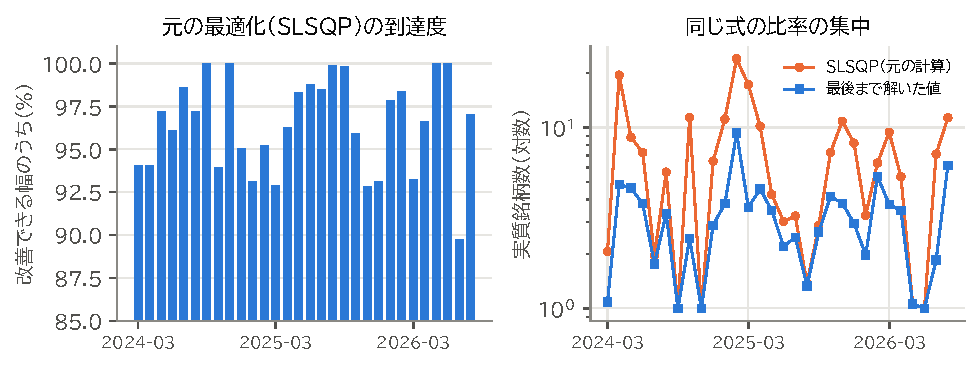
\includegraphics[width=0.95\linewidth]{h01_slsqp.pdf}
\caption{左：元の最適化が、改善できる幅の何 \% まで進んで止まったか。右：同じ目的関数の比率の集中（SLSQP の結果と、最後まで解いた結果）。}
\label{fig:slsqp}
\end{figure}

% ============================================================
\chapter{H02：LLM の数値予想と統計モデル}\label{ch:h02}

\begin{verdict}[判定：支持された]
LLM の予想を、判断月の平均日次リターンと散らばりの順位で回帰した残差（LLM に固有の部分）の IC は $-0.004$（$t$ $-0.28$、$p=0.78$、95\% 区間 $-0.036$〜$+0.027$）。区間の上限が意味のある最小の効果 0.03 を下回るので、「LLM に固有の予測力は、あっても IC 0.03 未満」と判定した。
\end{verdict}

\begin{figure}[htbp]
\centering
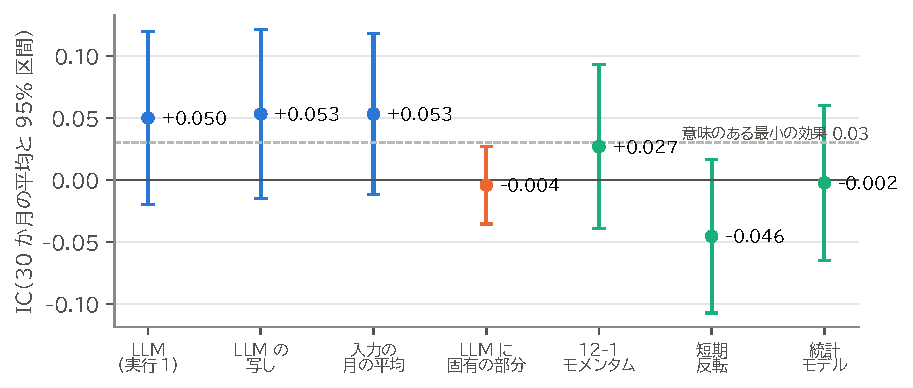
\includegraphics[width=0.95\linewidth]{h02_ic.pdf}
\caption{予想ごとの IC（30 か月の平均と 95\% 区間）。}
\label{fig:h02}
\end{figure}

\begin{table}[htbp]
\centering
\caption{予想の当たり具合（30 か月）。}
\small
\begin{tabular}{lrrr}
\toprule
予想 & IC の平均 & $t$ & 95\% 区間 \\
\midrule
LLM（実行 1） & $+0.050$ & 1.46 & $-0.020$〜$+0.120$ \\
LLM の写し（入力の平均と散らばりの回帰） & $+0.053$ & 1.60 & $-0.015$〜$+0.121$ \\
判断月の平均日次リターン（LLM が見た数字） & $+0.053$ & 1.68 & $-0.012$〜$+0.118$ \\
LLM に固有の部分 & $-0.004$ & $-0.28$ & $-0.036$〜$+0.027$ \\
12-1 か月のモメンタム & $+0.027$ & 0.83 & $-0.039$〜$+0.093$ \\
短期反転（$-$直近 1 か月） & $-0.046$ & $-1.51$ & $-0.107$〜$+0.016$ \\
統計モデル（12 指標のリッジ回帰、2015 年から学習） & $-0.002$ & $-0.08$ & $-0.065$〜$+0.060$ \\
\bottomrule
\end{tabular}
\end{table}

\begin{itemize}
\item 写しの決定係数は平均 0.81。LLM の予想の 8 割は、入力の月の平均と散らばりの直線の関数である。
\item LLM、写し、入力の平均そのものの IC はほぼ同じ。この期間に IC が少し正だったのは、直近 1 か月の値動きがわずかに続いたためで、LLM が足した情報ではない。
\item 統計モデルは、学習期間（2015〜）では指標の IC が小さく（資料）、評価期間でも当たらなかった。統計モデルと LLM の IC の差は $-0.052$（$t$ $-1.08$）で、区別できない。
\item MAE は LLM 0.45\%/日、写し 0.44\%/日、「0 と予想」0.33\%/日。LLM の予想の大きさは、何も予想しないより外れが大きい。方向の正解率は LLM 52.3\%、統計モデル 49.5\%。
\end{itemize}

% ============================================================
\chapter{H03：ビューの形（$q$ と $P$）}\label{ch:h03}

\begin{verdict}[判定：支持されなかった]
対角の $\Omega$・TE 3\% で、絶対ビューの「予想の水準」と「能動ベータ」の相関は $r=+0.71$（$p=1.3\times10^{-5}$）で、楽観の月ほど高ベータに傾くことは確かめられた。しかし、相対ビューの能動ベータの絶対値は絶対ビューの 0.94 倍で、条件（半分以下）を満たさなかった。
\end{verdict}

\begin{figure}[htbp]
\centering
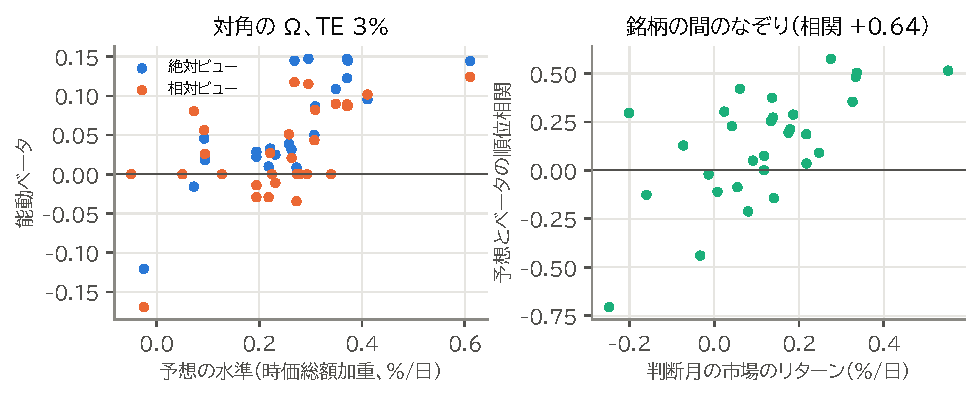
\includegraphics[width=0.95\linewidth]{h03_beta.pdf}
\caption{左：予想の水準と能動ベータ（30 か月）。右：判断日ごとの「LLM の予想と銘柄のベータの順位相関」と、判断月の市場のリターン。}
\label{fig:h03}
\end{figure}

\section{予想と違った点（探索的な診断）}

$\Omega\propto\Sigma$ では、相対ビューと絶対ビューの比率はすべての月で一致した（資料の結果の再確認）。それでも、水準と能動ベータの相関は $r=+0.62$ 残った。理論上、この場合は水準の上乗せは比率に効かないので、傾きの元は水準ではない。

\figref{fig:h03} の右のとおり、判断日ごとの「LLM の予想と銘柄のベータの順位相関」は、判断月の市場のリターンと $r=+0.64$ で連動した。市場が上がった月は高ベータの銘柄ほど上がっていて、LLM はそれをなぞるので、\textbf{銘柄の間の予想の差そのものが「高ベータが良い」という形になる}。予想の水準は市場のリターンと $r=+0.90$ で動くので、水準と能動ベータが相関して見えた。相対ビューは水準しか取り除かないので、この傾きは残る。取り除くには、ビューからベータの方向を取り除くか、能動ベータ 0 の制約を置く必要がある（\chapref{ch:next}）。これは事前に決めた検定ではないので、探索的な結果として扱う。

\section{順位ビューと成績}

TE 3\% の制約があると、順位ビューの最大の能動ウェイトは 1.40\%（絶対ビュー 1.44\%）で、ほとんど差がない。TE の制約がない場合、$\Omega\propto\Sigma$ の順位ビューは能動ベータ 0.13（絶対ビュー 0.20）、TE 17.5\%（同 24.1\%）で、外れ値の影響を少し抑えた。TE 3\% の 6 通りの超過リターンは $-0.4$\%〜$-0.7$\%（$|t|\le0.26$）で、時価総額加重と区別できない。

% ============================================================
\chapter{H04：$\Omega$ の設計と信頼度の較正}\label{ch:h04}

\begin{verdict}[判定：(3) 主な検定は支持、(2) 支持、(1) 棄却]
(3) 較正して縮めた $\Omega$ のコスト控除後の年率超過リターンは $+0.53\%$。予想を銘柄の間で並べ替えたビュー 200 回の平均は $-1.39\%$、95 パーセンタイルは $+1.14\%$、片側の経験的 $p=0.104$。ビューの情報は検出されない。(2) 実現の採用率は設定どおり（差 $5\times10^{-16}$）、実質 47.2 銘柄、実績の TE 4.2\%。(1) 回答のばらつきは、ボラティリティを統制しても外れの大きさと偏順位相関 $+0.17$（$t$ 12.9、30 か月すべて正）を持ち、予想と違って「外れやすさの順番」の手がかりになった。
\end{verdict}

\begin{figure}[htbp]
\centering
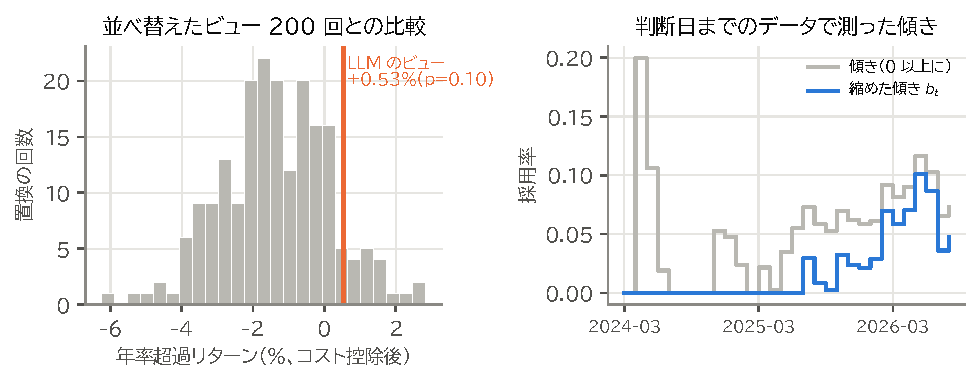
\includegraphics[width=0.95\linewidth]{h04_placebo.pdf}
\caption{左：並べ替えたビュー 200 回の超過リターンの分布と、実際の LLM のビュー。右：判断日までのデータで測った較正の傾き（灰）と、推定の誤差で縮めた値（青）。}
\label{fig:h04}
\end{figure}

\begin{table}[htbp]
\centering
\caption{$\Omega$ の 5 通り（相対ビュー、TE 3\%、コスト控除後、30 か月）。}
\label{tab:h04}
\small
\begin{tabular}{lrrrrrrr}
\toprule
$\Omega$ & 採用率 & 実質銘柄数 & 年率超過 & TE & IR & $t$ & 回転率 \\
\midrule
回答の分散（元の方法） & 87.6\% & 39.1 & $-0.2$\% & 5.1\% & $-0.05$ & $-0.08$ & 65\% \\
He--Litterman & 73.7\% & 39.5 & $+0.7$\% & 4.9\% & $+0.13$ & $+0.21$ & 61\% \\
傾きで較正（対角） & 28.2\% & 45.0 & $-0.6$\% & 4.0\% & $-0.15$ & $-0.24$ & 36\% \\
傾きで較正（$\Sigma$ に比例） & 5.3\% & 42.8 & $-0.4$\% & 5.1\% & $-0.07$ & $-0.12$ & 54\% \\
同上・傾きを縮める（主な戦略） & 0.0\%$^*$ & 47.2 & $+0.5$\% & 4.2\% & $+0.13$ & $+0.20$ & 31\% \\
主な戦略・翌取引日に売買 & --- & 47.2 & $+0.3$\% & 3.8\% & $+0.07$ & $+0.11$ & 31\% \\
\bottomrule
\end{tabular}
\par\smallskip{\footnotesize $^*$ 30 か月のうち 16 か月で $b_t=0$（傾きの $t$ 値が 1 未満）だったため中央値は 0。ビューが比率を動かしたのは 2025-07 以降の 14 か月で、$b_t$ は 0.002〜0.10。}
\end{table}

\begin{itemize}
\item TE の制約があると、$\Omega$ の決め方による成績の差はどれも偶然の範囲（$|t|\le0.24$）だった。違いが出るのは採用率と売買回転率で、較正して縮めるほど売買が減り、コスト負けが小さくなる。
\item 並べ替えたビューが平均で時価総額加重を下回るのは、情報のない傾きにもコストと TE のずれがかかるためである。実際のビューはその平均を 1.9 ポイント上回ったが、偶然と区別できない。
\item 回答のばらつきは、そのまま $\Omega$ に使うと確信が強すぎる（外れの 2 乗の約 8 分の 1）が、銘柄の間の外れやすさの順番には使える。『ビューとリスクのコツ』の「順番には使えるが、大きさは較正が要る」を、データで裏づけた。
\item 判断日の翌取引日に売買しても（感度分析）、結論は変わらない。
\item 最適化の状態は、主な戦略で 29 か月が最適、1 か月が「最適（精度が不十分の可能性）」だった。
\end{itemize}

% ============================================================
\chapter{H05：市場とセクターを、文章だけ・数字だけで聞く}\label{ch:h05}

\begin{verdict}[判定：なぞりが消えることは支持。当たるかどうかは証拠が不足]
文章だけ（T）では、市場の点数と \SP{} の直近 1 か月のリターンの順位相関が $+0.05$（$p=0.78$）で、G（文章＋数字）の $+0.77$ より有意に小さい（Fisher の $z$、$p=0.0004$）。セクターの IC は $+0.06$（$t$ 0.72、95\% 区間 $-0.11$〜$+0.24$）で、当たるとも当たらないとも言えない。
\end{verdict}

\begin{figure}[htbp]
\centering
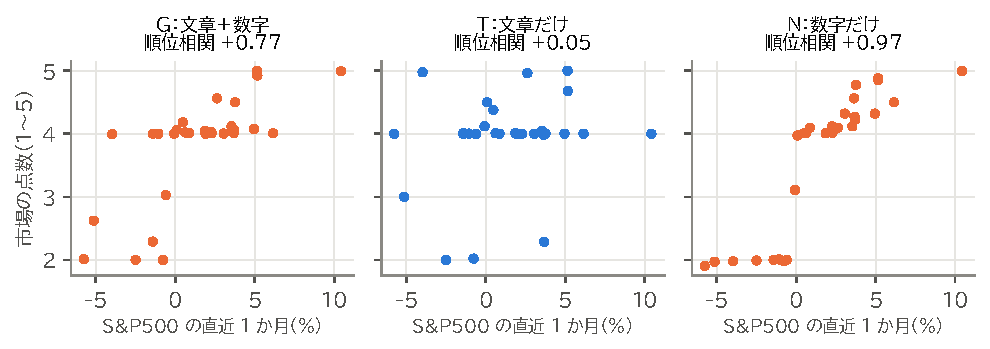
\includegraphics[width=0.98\linewidth]{h05_trace.pdf}
\caption{市場の点数と、\SP{} の直近 1 か月のリターン（30 か月）。左から G、T、N。}
\label{fig:h05}
\end{figure}

\begin{table}[htbp]
\centering
\caption{渡す情報による違い（30 か月）。}
\small
\begin{tabular}{lrrr}
\toprule
 & G：文章＋数字（既存） & T：文章だけ & N：数字だけ \\
\midrule
市場の点数と直近 1 か月のリターンの順位相関 & $+0.77$ & $+0.05$ & $+0.97$ \\
市場の点数と VIX の順位相関 & $-0.59$ & $-0.27$ & $-0.56$ \\
市場の点数の月ごとの標準偏差 & 0.84 & 0.73 & 1.11 \\
セクターの IC（$t$） & $-0.13$（$-1.64$） & $+0.06$（0.72） & $-0.13$（$-1.67$） \\
セクターの点数の平均（3 が指数と同じ） & 2.28 & 2.96 & 2.37 \\
\bottomrule
\end{tabular}
\end{table}

文章だけを渡すと、点数は月によって動く（標準偏差 0.73）が、市場の数字には沿わない。数字だけを渡すと、なぞりは G よりさらに強く（$+0.97$）、セクターの IC も G とほぼ同じだった。G の答えは、ほぼ渡した数字で決まっていた。数字はセクターの答えを悲観（2 点台）に傾けていた。

\textbf{設計からのずれ}：設計書には「温度 0 で確率を読む（G と同じ）」と書いたが、G は温度 1.0・30 回答で、最初のトークンの確率を使っていた。意図（G と同じ設定）に合わせて G の設定で行った。後から 30 件で温度 0 と 1 の確率を比べると、差の中央値は 0.002 とごく小さかったが、最大で 0.22（点数で 0.43）の差があった（\chapref{ch:review}）。同じ温度で聞き直したときのぶれと区別していないので、温度の影響かどうかは分からない。温度 1.0 にそろえた G・T・N の比較には影響しない。

% ============================================================
\chapter{H06：決算発表文から LLM が取り出す情報}\label{ch:h06}

\begin{verdict}[判定：支持されなかった]
合成点数（語調 + 見通し + ガイダンスの変更、学習なし）の Fama--MacBeth の係数は、売上と利益の前年比、直近 1 か月のリターン、12-1 か月のモメンタムを統制して $+0.017$（$t$ 0.97、$p=0.34$、95\% 区間 $-0.019$〜$+0.052$）。数値を統制しても残るとは言えない。区間は意味のある大きさ（0.03 以上）も含み、効果がないとも言えない。
\end{verdict}

\section{データ}

SEC EDGAR から、各社の 8-K（Item 2.02）に付く決算発表文（EX-99.1）を、提出日 2023-11-01〜2026-08-30 について取得した（522 社、6,209 本）。最初の規則で選んだ書類のうち約 270 本が補足資料や契約書だったので、文章の先頭に書かれた種類で確かめ、215 本を EX-99.1 に差し替えた。判断日ごとに、提出日が判断日より前で 120 日以内の最新の 1 本を使い、gpt-4o-mini に 5,429 本を読ませた（失敗 0、費用 3.31 ドル）。LLM には銘柄の数字を一切渡していない。

\begin{figure}[htbp]
\centering
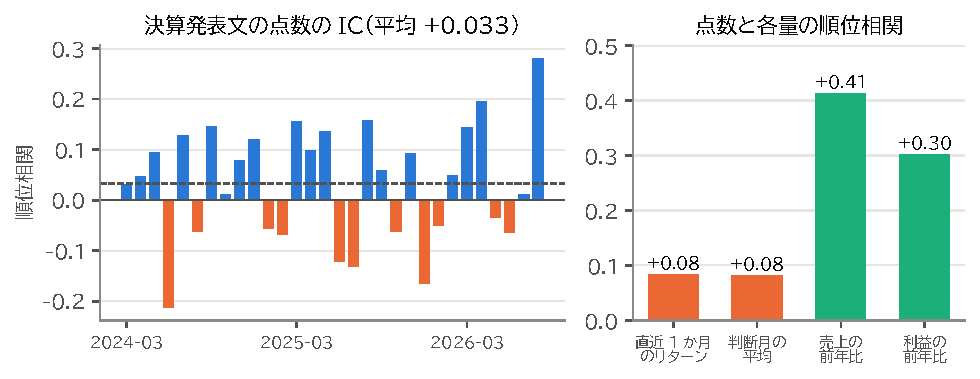
\includegraphics[width=0.95\linewidth]{h06_ic.pdf}
\caption{左：合成点数の月ごとの IC。右：合成点数と各量の順位相関（30 か月の平均）。}
\label{fig:h06}
\end{figure}

\begin{table}[htbp]
\centering
\caption{決算発表文の点数の当たり具合（参考。主な検定ではない）。}
\small
\begin{tabular}{lrrrr}
\toprule
 & IC の平均 & $t$ & $p$ & プラスの月 \\
\midrule
合成点数 & $+0.033$ & 1.57 & 0.13 & 19/30 \\
合成点数（発表から 35 日以内） & $+0.058$ & 1.59 & 0.12 & 20/30 \\
語調だけ & $+0.037$ & 1.93 & 0.064 & 19/30 \\
挙げたリスクの少なさ & $+0.011$ & 0.93 & 0.36 & 17/30 \\
\bottomrule
\end{tabular}
\end{table}

\begin{itemize}
\item \textbf{なぞりは起きない}：合成点数と直近 1 か月のリターンの順位相関は $+0.08$。売上の前年比とは $+0.41$、利益の前年比とは $+0.30$ で、点数は値動きではなく業績の文章に沿う。数値の予想（入力との相関 0.89）とは性質が違う。
\item \textbf{点数は楽観に偏る}：語調の 88\%、見通しの 76\% が前向き、ガイダンスは 42\% が「引き上げ」。順位で使うので IC には影響しない。
\item \textbf{ポートフォリオ}：同じ作り方（相対ビュー、$\Omega\propto\Sigma$、縮めた傾き、TE 3\%）で、決算発表文の点数のビューは年率 $-0.6\%$（TE 2.1\%、$t$ $-0.44$）。較正の傾きは縮める前は毎月正（0.02〜0.08）だったが、標準誤差と同じくらいの大きさで、縮めると 0 か小さな値になった。統計モデルは縮めた傾きが一度も正にならず、比率は時価総額加重と同じだった。
\end{itemize}

% ============================================================
\chapter{H07：フィードバックの LLM}\label{ch:h07}

\begin{verdict}[判定：結論を出すには証拠が不足している]
主な検定の F2（自分の過去の成績の要約を渡す）と F0（実行 1）の月ごとの IC の差は $+0.011$（$t$ 0.76、$p=0.45$、95\% 区間 $-0.018$〜$+0.040$、フィードバックのある 29 か月）。有意な改善はないが、区間の上限が 0.03 を超えるので、「上がらない」とも言えない。
\end{verdict}

\section{条件}

既存のコードにはフィードバックの LLM がないので、何を渡すと何が良くなるはずかを先に決め、100 銘柄（最初の判断日の銘柄から種 0 で選び、指数から外れた銘柄はその月から除く）$\times$ 30 か月で比べた。モデル、温度、回答の数、出力の形は実行 1 と同じである。

\begin{table}[htbp]
\centering
\caption{条件ごとの結果（フィードバックのある 29 か月の平均）。「変化 ÷ 雑音」は、F0 からの予想の変化の大きさを、同じプロンプトで聞き直したとき（F0$'$）の変化で割った値。}
\label{tab:h07}
\adjustbox{max width=\linewidth}{%
\begin{tabular}{lrrrrrrr}
\toprule
条件 & IC & 水準の偏り（\%/日） & 入力との相関 & 較正の傾き & 変化 ÷ 雑音 & 回答の標準偏差 & プラスの割合 \\
\midrule
F0：実行 1（フィードバックなし） & $+0.027$ & $+0.12$ & 0.89 & 0.03 & --- & 0.14\% & 76\% \\
F0$'$：同じプロンプトで聞き直し & $+0.035$ & $+0.11$ & 0.90 & 0.03 & 1.0 & 0.14\% & 74\% \\
F1：自分の前月の予想と実際 & $+0.038$ & $+0.17$ & 0.89 & 0.07 & 2.2 & 0.18\% & 80\% \\
F2：自分の過去の成績の要約 & $+0.037$ & $\mathbf{+0.29}$ & 0.76 & 0.09 & 4.0 & 0.20\% & 93\% \\
F3：別の役（見直す役）が直す & $+0.010$ & $+0.11$ & 0.81 & 0.03 & 2.5 & 0.11\% & 88\% \\
\bottomrule
\end{tabular}}
\end{table}

\begin{figure}[htbp]
\centering
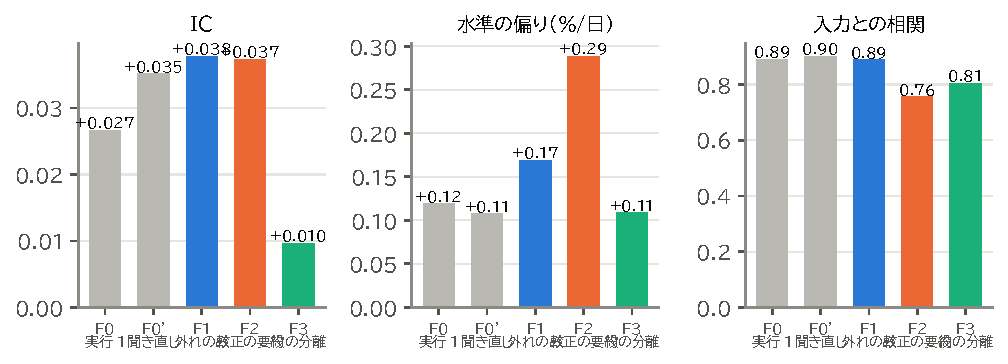
\includegraphics[width=0.98\linewidth]{h07_feedback.pdf}
\caption{条件ごとの IC、水準の偏り、入力との相関。}
\label{fig:h07}
\end{figure}

\section{結果}

\begin{itemize}
\item \textbf{聞き直すだけで、IC はこのくらい動く。}F0$'$ と F0 の IC の差は $+0.009$（$t$ 1.61）。フィードバックの効果を論じるには、この雑音の幅との比較が欠かせない。
\item \textbf{F1（前月の外れ）}：予想を雑音の目安の 2.2 倍動かした（外れを追いかける過剰な反応）が、IC は F0 と区別できない（差 $+0.011$、$t$ 1.46）。
\item \textbf{F2（成績の要約）}：予想と違い、楽観の偏りが日次 $+0.12\%$ から $+0.29\%$ に大きくなり、プラスの予想が 93\% になった。予想は同じ月の F0 とほぼ並行に動き（相関 0.96）、どの月も一律に約 $+0.17\%$/日 上振れした。要約に書いた「あなたの予想の平均 0.0031〜0.0035/日、実際 0.0000〜0.0007/日」を、LLM は「高すぎた」という警告ではなく、一律に強気に寄せる方向に受け取った。上振れした予想は次の月の要約の平均になるので、自己参照の形になっている。ただし、月を追って増幅するほどの連動は見られなかった（上振れの大きさと要約の数値の相関 $+0.19$、市場の動きとは $-0.04$、\chapref{ch:review}）。
\item \textbf{F3（役の分離）}：偏りはほぼ変わらず（$+0.11\%$）、IC はむしろ下がる方向だった（差 $-0.017$、$t$ $-1.54$）。予想の幅は小さくなった（回答の標準偏差 0.11\%）。
\item \textbf{なぞり}：F2 と F3 は入力との相関を 0.89 から 0.76・0.81 に少し下げた。要約の「入力の平均と相関している」という一文が効いた可能性がある。
\end{itemize}

\section{BLM への意味}

フィードバックで良くなると期待したもの（水準の偏り）は、相対ビューと $\Omega\propto\Sigma$ のもとでは比率に効かない（H03、H04）。つまり、BLM の側で取り除ける。逆に、F2 で悪化した偏りは、絶対ビュー・対角の $\Omega$ で使えば高ベータへの傾きを強める。数字の成績を LLM に渡して直させる形のフィードバックは、この研究の範囲では、予想の当たり具合を確かめられるほど上げず、自己強化と過剰な反応という副作用を示した。設計書で「BLM 適用後の比率やリスクを渡す」条件を行わなかった判断は、この結果を見ても変えない（比率の情報で予想の何が良くなるべきかを、事前に決められないため）。

% ============================================================
\chapter{対照群と実験群の比較}\label{ch:compare}

\section{予想の当たり具合}

\begin{table}[htbp]
\centering
\caption{同じ 30 か月・同じ銘柄の予想の IC（銘柄ごとの予想。月ごとの順位相関の平均）。}
\small
\begin{tabular}{llrrr}
\toprule
区分 & 予想 & IC & $t$ & 出典 \\
\midrule
LLM（数値） & 実行 1（既存） & $+0.050$ & 1.46 & H02 \\
LLM を使わない & 判断月の平均日次リターン & $+0.053$ & 1.68 & H02 \\
LLM を使わない & 統計モデル（リッジ） & $-0.002$ & $-0.08$ & H02 \\
LLM を使わない & 12-1 か月のモメンタム & $+0.027$ & 0.83 & H02 \\
LLM（文章） & 決算発表文の合成点数 & $+0.033$ & 1.57 & H06 \\
LLM（文章） & 同、発表から 35 日以内 & $+0.058$ & 1.59 & H06 \\
\bottomrule
\end{tabular}
\end{table}

\section{ポートフォリオ}

\begin{table}[htbp]
\centering
\caption{主な戦略の成績（30 か月、コスト控除後、時価総額加重との差は年率）。}
\label{tab:portfolios}
\adjustbox{max width=\linewidth}{%
\begin{tabular}{lrrrrrrrrr}
\toprule
戦略 & 年率 & リスク & シャープ & 最大下落 & 超過 & TE & IR & $t$ & 回転率 \\
\midrule
時価総額加重（ビューなし） & 17.7\% & 12.2\% & 1.06 & $-7.7$\% & --- & --- & --- & --- & 0\% \\
LLM 数値・回答の分散の $\Omega$ ＋ TE 3\% & 17.2\% & 13.7\% & 0.93 & $-8.6$\% & $-0.2$\% & 5.1\% & $-0.05$ & $-0.08$ & 65\% \\
LLM 数値・較正して縮めた $\Omega$ ＋ TE 3\% & 18.2\% & 12.8\% & 1.05 & $-7.7$\% & $+0.5$\% & 4.2\% & $+0.13$ & $+0.20$ & 31\% \\
同、翌取引日に売買 & 17.8\% & 12.7\% & 1.03 & $-7.8$\% & $+0.3$\% & 3.8\% & $+0.07$ & $+0.11$ & 31\% \\
並べ替えたビュー 200 回（平均） & --- & --- & --- & --- & $-1.4$\% & 2.5\% & --- & --- & --- \\
決算発表文の点数・同じ作り方 & 17.0\% & 12.4\% & 1.00 & $-8.0$\% & $-0.6$\% & 2.1\% & $-0.28$ & $-0.44$ & 31\% \\
統計モデル・同じ作り方$^*$ & 17.7\% & 12.2\% & 1.06 & $-7.7$\% & 0.0\% & 0.0\% & --- & --- & 0\% \\
LLM 数値・較正した $\Omega$、TE の制約なし & 30.5\% & 27.6\% & 0.96 & $-21.7$\% & $+13.4$\% & 24.1\% & $+0.56$ & $+0.88$ & 79\% \\
\bottomrule
\end{tabular}}
\par\smallskip{\footnotesize $^*$ 較正の傾きが一度も正にならず、比率は時価総額加重と同じ。結果のファイルの IR 1.71 は 0 に近い差の割り算から出た数値の誤差である。}
\end{table}

\begin{figure}[htbp]
\centering
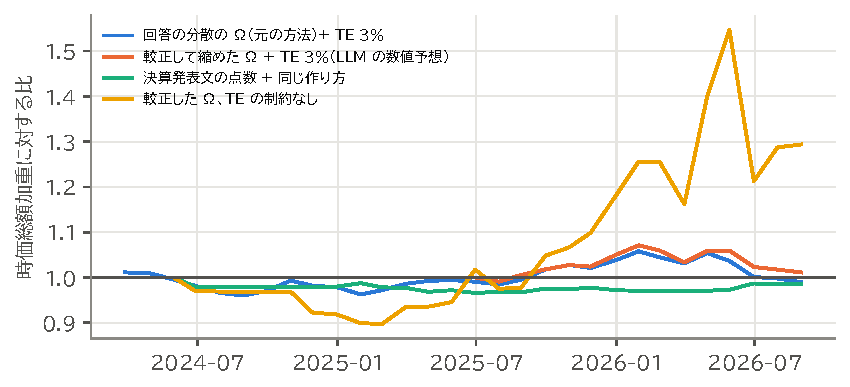
\includegraphics[width=0.92\linewidth]{cumulative.pdf}
\caption{時価総額加重に対する累積の比（コスト控除後）。}
\label{fig:cum}
\end{figure}

TE の制約がある戦略は、どれも時価総額加重と区別できない（$|t|\le0.44$）。TE の制約がない較正した戦略は、年率 $+13.4\%$ と大きく見えるが、TE 24\% で $t$ 値は 0.88 にとどまり、最大下落は時価総額加重の約 3 倍である。この数字を成果とは読めない（総合報告書の「結果が良すぎる」への備えと同じ）。

% ============================================================
\chapter{API の利用量と費用}\label{ch:cost}

\begin{table}[htbp]
\centering
\caption{実験で使った API（gpt-4o-mini、入力 100 万トークンあたり 0.15 ドル、出力 0.60 ドルで計算。全リクエストを \code{results/*.jsonl} に記録）。}
\label{tab:cost}
\small
\begin{tabular}{lrrrr}
\toprule
実験 & リクエスト & 入力トークン & 出力トークン & 費用（ドル） \\
\midrule
H05 文章だけ（T） & 540 & 103,782 & 16,200 & 0.025 \\
H05 数字だけ（N） & 540 & 154,508 & 16,200 & 0.033 \\
H06 決算発表文の読み取り & 5,429 & 21,443,558 & 162,118 & 3.314 \\
H07 F0$'$（聞き直し） & 2,917 & 1,398,390 & 1,186,858 & 0.922 \\
H07 F1（前月の外れ） & 2,917 & 1,499,802 & 1,012,707 & 0.833 \\
H07 F2（成績の要約） & 2,917 & 1,611,496 & 1,098,408 & 0.901 \\
H07 F3（役の分離） & 2,917 & 1,384,970 & 799,419 & 0.687 \\
追加の確認（H05 の温度） & 60 & 11,558 & 60 & 0.002 \\
\midrule
合計 & 18,237 & 27,608,064 & 4,291,970 & \textbf{6.717} \\
\bottomrule
\end{tabular}
\end{table}

\begin{itemize}
\item 失敗したリクエストは 0 件。再試行は OpenAI のクライアントが行い（上限 6 回、1 回の待ち時間の上限 60 秒）、重複したリクエストは送っていない（途中から再開するとき、回答済みのリクエストは飛ばす）。
\item 設計のレビューに gpt-5.5（入力 20,007、出力 2,695 トークン）と gemini-3.1-pro-preview（入力 17,863、出力 822 ＋ 思考 2,497 トークン）、コードのレビューに gpt-5.3-codex（入力 6,659、出力 14,700 トークン）、結果の考察に gpt-5.3-codex（入力 9,710、出力 5,148）と gemini-3.1-pro-preview（入力 9,215、出力 2,216 ＋ 思考 3,226）を使った。これらは予想には使っていない。単価を確かめていないので費用には含めていない（トークン数から見て、合わせて 1 ドル程度と見込む）。
\item 決算発表文の取得（SEC EDGAR）は無料。毎秒 8 回以下に抑え、連絡先を User-Agent に入れた（連絡先は実行時の環境変数で渡し、ファイルには残していない）。
\end{itemize}

% ============================================================
\chapter{別のモデルによる考察と、追加の確認}\label{ch:review}

H07 までの判定のメモ（\code{experiments/H0x/results/findings.md}）を、gpt-5.3-codex と gemini-3.1-pro-preview に読ませ、「別の説明」「言い過ぎや分析の誤り」「全体として何が言えるか」「次の実験」「見落としている発見」を挙げさせた（回答の全文は \code{experiments/robustness/results/external\_review.md}）。指摘は自分で確かめ、計算で確かめられるものは追加の確認を行った。\textbf{この章の追加の確認は、結果を見た後に行った探索的なもので、事前に決めた判定は変えない。}コードは \code{experiments/robustness/run.py}、結果は同じフォルダの \code{results/}。

\section{追加の確認}

\begin{table}[htbp]
\centering
\caption{月ごとの値の自己相関を考慮した Newey--West の $t$ 値（ラグ 3）。}
\label{tab:nw}
\small
\begin{tabular}{lrrrrr}
\toprule
系列 & 平均 & 通常の $t$ & Newey--West の $t$ & $p$ & 1 次の自己相関 \\
\midrule
H02 LLM に固有の部分の IC & $-0.004$ & $-0.28$ & $-0.29$ & 0.774 & $-0.11$ \\
H02 LLM の IC & $+0.050$ & 1.46 & 1.76 & 0.089 & $-0.08$ \\
H06 合成点数の係数（主な検定） & $+0.017$ & 0.97 & 1.41 & 0.168 & $-0.35$ \\
H06 合成点数の IC & $+0.033$ & 1.57 & \textbf{2.32} & \textbf{0.028} & $-0.15$ \\
H06 合成点数の IC（35 日以内） & $+0.058$ & 1.59 & \textbf{2.19} & \textbf{0.037} & $-0.01$ \\
H07 IC の差（F2 $-$ F0） & $+0.011$ & 0.76 & 0.84 & 0.406 & $+0.06$ \\
\bottomrule
\end{tabular}
\end{table}

\begin{description}[leftmargin=2em,style=nextline,itemsep=0.4em]
\item[自己相関（codex の指摘）] 月ごとの IC に自己相関があると、通常の $t$ 値はずれる。Newey--West の $t$ 値で計算し直すと（\tabref{tab:nw}）、H02 と H07 の結論は変わらない。H06 の主な検定（数値を統制した係数）も有意にならない（$t$ 1.41）。一方、決算発表文の合成点数そのものの IC は、負の自己相関のため通常の $t$ 値が小さく出ていて、Newey--West では $t$ 2.32（$p=0.028$）、発表から 35 日以内では $t$ 2.19 になった。\textbf{文章からの点数には、翌月のリターンとの弱い正の関係がある可能性が高い。ただし、それが売上や利益の伸びなどの数値を超える情報かどうかは確かめられていない。}多重比較の補正はしていない。また、30 個の観測で Newey--West の分散を推定すること自体の不確かさも大きい。
\item[置換の作り方（両モデルの指摘）] 全銘柄の間で予想を並べ替えると、セクターの構成やリスクの性質まで壊れ、比べる相手として弱すぎるおそれがある。セクターの中だけで並べ替える厳しい対照を 100 回作った（較正の傾きは実際の予想のもの）。並べ替えたビューの年率超過リターンは平均 $-0.17\%$、95 パーセンタイル $+2.52\%$ で、実際の LLM のビュー（$+0.53\%$）の片側 $p$ は 0.38 だった。全銘柄の置換（平均 $-1.39\%$）に対する 1.9 ポイントの差は、ほとんどがセクターの構成を保ったことで説明できる。\textbf{LLM のセクターの中での銘柄の順位には、情報が見られない。}置換の作り方を厳しくしても、H04 の判定は変わらない。
\item[置換の $p$ 値の誤差（codex の指摘）] 200 回の置換による $p=0.104$ には、モンテカルロの誤差（標準誤差 0.022、95\% で約 $\pm0.04$）がある。判定（$p\ge0.05$）は変わらない。
\item[H05 の温度（codex の指摘）] 30 件で温度 0 と 1 の確率を比べると、差の中央値は 0.002 とごく小さかったが、最大で 0.22（点数で 0.43）だった。「温度の影響を受けない」は言い過ぎだったので、\chapref{ch:h05} の記述を直した。
\item[H07 の楽観の原因（両モデルの指摘）] 「要約の中の自分の平均をなぞった」（私の最初の解釈）、「要約の統計量の書き方が上向きの目安になった」（codex）、「上昇相場に引っ張られた」（gemini）の 3 つの説明を比べた。F2 の月平均の予想は、同じ月の F0 とほぼ並行（相関 0.96）で、どの月も一律に約 $+0.17\%$/日 上振れした。上振れの大きさは、要約に書いた数値と相関 $+0.19$、判断月の市場の動きとは $-0.04$ だった。\textbf{市場に引っ張られた説明は支持されない。要約を見せること自体で一律に強気に寄る（目安として働く）という説明が最も合う。}
\end{description}

\section{採らなかった指摘と、その理由}

\begin{itemize}
\item \textbf{「Fama--MacBeth は銘柄の間の相関を統制していない」}（gemini）：Fama--MacBeth は、月ごとの断面回帰の係数を時系列で集計して、銘柄の間の相関の影響を除く方法である。指摘は当たらない。
\item \textbf{「H03 の傾きは、有名企業を好む LLM の固定的な偏りかもしれない」}（gemini）：傾き（予想とベータの順位相関）は、判断月の市場のリターンと $+0.64$ で月ごとに動く。固定的な偏りでは説明できない。
\item \textbf{「H03 の傾きは、ビューではなく最適化（制約と共分散の誤差）から来ているかもしれない」}（codex）：最適化の前のビューそのものが、ベータと月ごとに相関している（\figref{fig:h03} の右）。最適化が傾きを強めている可能性は残るが、元はビューにある。
\item \textbf{「回答のばらつきとボラティリティの相関（$+0.59$）は、LLM が不確実性を把握している証拠」}（gemini）：LLM は入力で判断月の日次リターンの列を見ているので、その散らばりをなぞっているだけの可能性が高い。H04 (1) の偏順位相関（ボラティリティを統制しても $+0.17$）は事実だが、統制に使ったのは過去 252 日のボラティリティで、LLM が見た 1 か月の散らばりではない。「LLM が不確実性を理解している」とまでは言えない。
\end{itemize}

\section{取り入れた考察}

\begin{itemize}
\item \textbf{BLM の較正は「LLM の価値を引き出す道具」ではなく「価値のないビューを無害にする安全装置」として働いた}（codex、gemini）。H04 の成績の差は、ビューの情報ではなく、売買の量とコスト負けの抑制から来ている。
\item \textbf{聞き直しの雑音と、プロンプトを変えた効果を必ず並べる}（codex）。H07 では、聞き直すだけで IC が $+0.009$ 動いた。プロンプトの工夫の効果を主張するには、この幅を超える必要がある。
\item \textbf{実績の TE が事前の目標を上回り続ける}（codex）：成績の評価には、ビューの良し悪しだけでなく、リスクモデル（252 日の縮小推定）の予測の誤差が入っている。
\item \textbf{LLM の数値予想は「雑音」ではなく「決まった向きに外す」}（gemini）：MAE が「0 と予想する」より大きく、楽観と直近のなぞりという決まった向きの誤差を持つ。そのまま使うと、比率を不要に動かす。
\item \textbf{決算発表文を、月次ではなく発表ごとのイベントとして評価する}（codex）：発表ごとに 1・5・20 日後の超過リターンを見れば、観測の数が月次の 10 倍以上になり、30 か月でも小さな効果を検出できる可能性がある（\chapref{ch:next}）。
\end{itemize}

% ============================================================
\chapter{仮説ごとの判定}\label{ch:verdicts}

\begin{table}[htbp]
\centering
\caption{仮説ごとの判定。主な検定の $p$ 値（両側）と、6 つの主な検定（H02〜H07）に Holm の補正をかけた値。H04 は置換の片側 $p=0.104$ の 2 倍。H03 の $p$ は「絶対ビューで水準と能動ベータが相関する」の部分（判定にはもう 1 つの条件がある）。}
\label{tab:verdicts}
\adjustbox{max width=\linewidth}{%
\begin{tabular}{llp{6.2cm}rrl}
\toprule
ID & 名称 & 主な検定と結果 & $p$ & Holm & 判定 \\
\midrule
H01 & 計算の整合性 & 式・単位・収束・先読みの確認と、資料の数値の再現 & --- & --- & 整合している（元の SLSQP は再現できない） \\
H02 & LLM と統計モデル & LLM に固有の部分の IC $-0.004$（区間 $-0.036$〜$+0.027$） & 0.783 & 1.000 & 支持された \\
H03 & ビューの形 & 水準と能動ベータの相関 $+0.71$。相対ビューの能動ベータは 0.94 倍（条件は 0.5 以下） & $1.3\times10^{-5}$ & $7.9\times10^{-5}$ & 支持されなかった \\
H04 & $\Omega$ の較正 & 超過 $+0.53\%$、置換 200 回の中で片側 $p=0.104$ & 0.209 & 1.000 & 支持された（(1) は棄却） \\
H05 & 文章だけ・数字だけ & なぞり $+0.77\to+0.05$（Fisher $p=0.0004$）。セクターの IC $+0.06$ & 0.475 & 1.000 & なぞりが消えることは支持。当たるかは証拠不足 \\
H06 & 決算発表文 & 数値を統制した係数 $+0.017$（$t$ 0.97） & 0.340 & 1.000 & 支持されなかった \\
H07 & フィードバック & IC の差（F2 $-$ F0）$+0.011$（区間 $-0.018$〜$+0.040$） & 0.455 & 1.000 & 証拠不足 \\
\bottomrule
\end{tabular}}
\end{table}

依頼の 4 区分に当てはめると次のとおりである。実験未実施の仮説はない。

\begin{itemize}
\item \textbf{支持された}：H02（LLM の数値予想に固有の予測力は、あっても IC 0.03 未満）、H04 の主な検定（較正した BLM のビューは、並べ替えたビューと区別できない）と (2)（較正した BLM は設計どおりに動く）、H05 の前半（文章だけでなぞりが消える）。
\item \textbf{支持されなかった}：H03（相対ビューではベータの傾きが消えない）、H04 の (1)（回答のばらつきは外れやすさの順番を持つ）、H06（決算発表文の点数が数値を超える情報を持つことは示せない）。
\item \textbf{結論を出すには証拠が不足している}：H05 の後半（文章の判断が当たるか）、H07（フィードバックで IC が上がるか）。H06 も、信頼区間が意味のある大きさを含むので、実質的には「証拠が不足している」に近い。
\item \textbf{実験未実施}：なし。ただし H07 の「BLM 適用後の比率やリスクを渡す」条件は、設計の段階で行わないと決めた。
\end{itemize}

Holm の補正の後に 5\% で有意なのは H03 の相関だけである。「LLM のビューに予測力がある」という向きの主張は、補正の前でも、どの仮説でも有意にならなかった。

% ============================================================
\chapter{失敗した実験、設計からのずれ、その原因}\label{ch:failures}

\begin{longtable}{p{3.8cm}p{11.1cm}}
\toprule
\textbf{事柄} & \textbf{内容と対処} \\
\midrule
\endfirsthead
\bottomrule
\endfoot
元の計算の再現 & SLSQP の結果は入力のわずかな違いで変わり、保存された比率と一致しなかった（H01）。研究の仮説とは分け、以降の比較では元の計算を使わなかった \\
H03 の予想の外れ & 「水準の癖が能動ベータに入り、相対ビューで消える」と予想したが、傾きは銘柄の間のなぞりから来ていて、相対ビューでは消えなかった \\
H04 の (1) の予想の外れ & 回答のばらつきは外れの順番の手がかりにならないと予想したが、統制後も偏順位相関 $+0.17$ が残った \\
H04 の計算時間 & 置換 200 回の並列計算で、各プロセスが数十のスレッドを立てて CPU を取り合い、最初の実行が非常に遅くなった。途中で止め、1 プロセス 1 スレッドにして計算し直した（乱数の種は固定なので結果は同じ）。GPU も検討したが、時間の 9 割は CPU で動く最適化のソルバーで、GPU 化には解き方を替える必要があるので採らなかった \\
H05 の温度 & 設計書の「温度 0」は転記の誤りで、意図どおり G と同じ温度 1.0 で行った。また「温度の影響を受けない」と書いたのは言い過ぎだった（\chapref{ch:review}） \\
H07 の予想の外れと計算時間 & 「要約を渡すと楽観が減る」と予想したが、逆に増えた。また、F2・F3 に渡す要約を銘柄ごとに作り直していて遅かったので、月に 1 回だけ作るように直して再開した（要約の中身は同じで、回答済みのリクエストは飛ばした） \\
H06 の書類の選び方 & 最初の規則で約 270 本が EX-99.1 でなかった。種類を確かめて 215 本を差し替えた。4 本は EX-99.1 が見つからず、72 本は書類がなかった \\
H06 の記録の大きさ & 読み取りの記録（\code{scores.jsonl}、91MB）に決算発表文の本文がそのまま入り、Git にコミットしてプッシュした。設計書の「文章は Git に入れない」と食い違う。履歴から消すには強制プッシュが要るので行っていない（\chapref{ch:next}） \\
\end{longtable}

% ============================================================
\chapter{データ・期間・評価方法による限界}\label{ch:limits}

\begin{itemize}
\item \textbf{評価は 30 か月だけ。}IC の月ごとの標準偏差が約 0.19 なので、$t$ 値 2 に届くのは IC 0.07 以上である。決算発表文の点数（IC 0.03〜0.06）のような小さな効果は、本当にあっても検出できない。H06 の結論は「効果がない」ではなく「確かめられない」である。
\item \textbf{相場の局面。}評価期間は上昇相場が中心で、下落相場での挙動は分からない。
\item \textbf{生存者バイアス。}データの取れない 28 銘柄の除外は全戦略に共通で、比較は公平だが、成績の水準には偏りが残る。
\item \textbf{モデルは 1 つ。}予想に使ったのは gpt-4o-mini だけである。新しいモデルは評価期間の相場を学習で知っている可能性があり、使えない。
\item \textbf{既存のデータの再分析。}H02〜H04 は、全体の当たり具合（IC $+0.05$ など）を知ったうえでの分析である。指標と判定の基準は分析の前に固定したが、何も知らない状態の事前登録ではない。
\item \textbf{多重比較。}主な検定は 6 つで、Holm の補正をかけた。副次の結果は参考で、多重比較の補正はしていない。
\item \textbf{取引コスト。}片道 0.1\% だけを入れた。売買の価格への影響（マーケットインパクト）は入れていない。
\item \textbf{事前の TE と実績の TE。}事前 3\% に対して、実績は 4〜5\% だった。
\end{itemize}

% ============================================================
\chapter{次に行うべき実験}\label{ch:next}

\begin{enumerate}
\item \textbf{決算発表文の点数を、発表ごとのイベントとして確かめる。}月次の断面ではなく、発表ごとに 1・5・20 日後の（市場やセクターに対する）超過リターンを目的にする。観測の数が数千になり、知識の期限の後の期間（2023 年 11 月以降）のままで、小さな効果を検出できる可能性がある。点数は今回のもの（5,429 本）をそのまま使えるので、API の費用はかからない。今回いちばん有望だった結果（Newey--West で $t$ 2.32）を、事前に決めた検定で確かめ直すことにもなる。
\item \textbf{決算発表文の点数を、期間を延ばして確かめる。}IC $+0.03$〜$+0.06$ を検出するには 50〜60 か月以上が要る。EDGAR の 8-K は 2010 年代から取れるが、gpt-4o-mini の知識の期限（2023 年 10 月）より前の文章では、モデルがその後の株価を知っているおそれがある。社名と数字を伏せた文章で、知識の期限の前と後の当たり具合を比べる（Kim ほか 2024 の匿名化と同じ考え方）。
\item \textbf{ビューからベータの方向を取り除く。}H03 で見つかった傾きを、判断日ごとに予想をベータで回帰した残差を使う形と、能動ベータ 0 の制約の 2 通りで取り除き、TE と成績への影響を見る。
\item \textbf{回答のばらつきを、順番の情報として使う。}H04 で、ばらつきは外れやすさの順番を持っていた。$\Omega$ の大きさは較正の傾きで決め、銘柄の間の相対的な大きさだけをばらつきの順位で変える形を試す。
\item \textbf{統計モデルを直す。}評価期間の前（2015〜2024）でも指標の IC が小さく、リッジは当たらなかった。セクターの中での順位、業種ごとの指標、決算の驚き（予想との差）など、文献で効果が報告されている変数を試す。
\item \textbf{条件を固定した前向きの記録。}モデル、プロンプト、$\Omega$、最適化を固定し、判断日ごとの入力のスナップショットとともに、これから毎月の予想を記録する。期間を延ばす方法として、未来の情報や後からの調整の疑いが最も少ない。
\item \textbf{DB への記録。}実験の結果は今はファイル（CSV、JSONL）にある。今後も使う結果は、既存の行を変えずに新しいテーブル（実験の条件と、判断日・銘柄ごとの回答と点数）に取り込み、\code{llm\_runs} にユーザープロンプトの型と条件の列を足す。
\item \textbf{Git の履歴の整理。}\code{experiment/H06-earnings-text} 以降のブランチに入った 91MB の記録（決算発表文の本文を含む）を、履歴から消すかどうかを決める。消すには強制プッシュが要る。
\end{enumerate}

% ============================================================
\chapter{推奨するアーキテクチャ}\label{ch:recommend}

\begin{figure}[htbp]
\centering
\begin{tikzpicture}[node distance=5mm and 5mm]
\node[box=c3] (txt) {銘柄ごとの文章\\{\scriptsize 決算発表文など。公表日つき}};
\node[box=c2,right=of txt] (llm) {LLM\\{\scriptsize 文章から点数を取り出す。数字は渡さない}};
\node[box=c1,right=of llm] (cal) {較正\\{\scriptsize 判断日より前の点数と結果で傾き $b_t$。誤差で縮める}};
\node[box=c4,right=of cal] (bl) {BLM\\{\scriptsize 相対ビュー、$\Omega\propto\Sigma$、採用率 $b_t$}};
\node[box=c1,below=of bl] (opt) {最適化\\{\scriptsize TE の上限、（能動ベータの制約）}};
\node[box=c3,below=of txt] (num) {数値のデータ\\{\scriptsize 株価、財務、市場}};
\node[box=c1,right=of num] (stat) {統計モデル\\{\scriptsize 同じ較正の決まりで比べる}};
\draw[arr] (txt) -- (llm); \draw[arr] (llm) -- (cal); \draw[arr] (cal) -- (bl); \draw[arr] (bl) -- (opt);
\draw[arr] (num) -- (stat); \draw[arr] (stat) -| (cal);
\end{tikzpicture}
\caption{推奨する構成。LLM は文章の解釈だけを受け持ち、数値化と信頼度は過去の結果から統計で決める。}
\label{fig:recommend}
\end{figure}

\begin{enumerate}
\item \textbf{LLM に数値のリターンを予想させない。}数値の予想は入力の写しで（H02）、BLM の中でもベータの傾きとして入り込む（H03）。数値の情報は統計モデルで扱い、その比べる相手として残す。
\item \textbf{LLM の役割を、文章からの情報の取り出しに絞る。}文章だけを渡すと、なぞりは消え（H05、H06）、点数は業績の内容に沿う。点数は「語調・見通し・ガイダンス」のような、記録して当たり具合を測れる形で取り出す。
\item \textbf{信頼度は LLM に言わせず、過去の結果から測る。}$\Omega\propto\Sigma$ で、採用率を判断日より前の較正の傾き（推定の誤差で縮めたもの）にすると、BLM は設計どおりに働き、当たっていないビューは自動で使われなくなる（H04）。回答のばらつきは、順番の手がかりとしてだけ使う。
\item \textbf{比率の大きさは TE の上限で決める。}$\tau$ で TE を合わせない。実績の TE は事前の目標を上回るので、目標は控えめに置く。
\item \textbf{フィードバックの LLM は、予想の改善の道具としては入れない。}数字の成績を渡すと、楽観が強まり、前月の外れを追いかけた（H07）。水準の偏りは BLM の側（相対ビューと較正した $\Omega$）で取り除く。フィードバックを入れるなら、総合報告書の段階 2 の計画どおり、数字での要因の分解を説明させる役（予想を変えない役）にとどめる。
\item \textbf{評価は置換の対照と一緒に行う。}成績は、情報のないビュー（並べ替え）と比べて初めて読める（H04）。
\end{enumerate}

この構成を採る理由は、成績が最も高かったからではない（30 か月では、どの方法も時価総額加重と区別できない）。(a) 予想の当たり具合と比率の動きが対応していて説明できる、(b) 当たらないビューが自動で無害になる、(c) 費用が小さい（決算発表文 1 本あたり約 0.06 セント）、(d) 未来の情報が混ざる経路が少ない、の 4 点で、既存の構成より優れているためである。LLM が追加の価値を生むかどうかは、この構成で期間を延ばして確かめる必要がある。

% ============================================================
\appendix
\chapter{ブランチとコミット}\label{app:branches}

各ブランチは 1 つ前のブランチから分岐している（設計書は \code{db-from-2015} から）。すべて \code{origin}（\code{sumataro0840/LLM-BLM}）にプッシュした。強制プッシュはしていない。

\begin{table}[htbp]
\centering
\small
\begin{tabular}{lll}
\toprule
内容 & ブランチ & コミット \\
\midrule
設計書 & \code{research/llm-blm-hypotheses} & \code{95e184d} \\
H01 計算の検証と共通の部品 & \code{experiment/H01-verification} & \code{091eb19} \\
H02 統計モデル & \code{experiment/H02-statistical-baseline} & \code{1ae3ed6} \\
H03 ビューの形 & \code{experiment/H03-view-shape} & \code{887c451} \\
H04 $\Omega$ の較正 & \code{experiment/H04-omega-calibration} & \code{3f661b3} \\
H05 文章だけ・数字だけ & \code{experiment/H05-text-vs-numbers} & \code{9b6a7c8} \\
H06 決算発表文 & \code{experiment/H06-earnings-text} & \code{d357677} \\
H07 フィードバック & \code{experiment/H07-feedback-llm} & \code{b26ea10} \\
本書と追加の確認 & \code{research/llm-blm-results-report} & （本書を含むコミット） \\
\bottomrule
\end{tabular}
\end{table}

レビューの記録（フォルダ \code{experiments/robustness/results/}）：
\begin{itemize}
\item 設計書の最初の版へのレビュー：\code{external\_review\_design.md}
\item 共通部品のコードへのレビュー：\code{external\_review\_code.md}
\item 結果の考察：\code{external\_review.md}
\end{itemize}

\end{document}
